\documentclass[12pt, a4paper]{article}
\usepackage[labelfont=bf]{caption}
\usepackage{fancyhdr}
\usepackage{float}
\usepackage[top=25mm, right=25mm, bottom=20mm, left=25mm]{geometry}
\usepackage[hidelinks]{hyperref}
\usepackage{multicol}
\usepackage{parskip}
\usepackage{pgfplots}

\pagestyle{fancy}
\fancyhead[L]{COM3110}
\fancyhead[C]{Assignment: Document Retrieval}
\fancyhead[R]{Zer Jun Eng}

\pgfplotsset{small, height=8cm, compat=1.9}

\begin{document}

\section{Implementation of Weighting Scheme}
\subsection{Binary}
The binary scheme is fully implemented. The term weight is either 1 or 0. For every candidate
document, $q_i d_i$ is the number of common terms that appear in both query and the document, and
$d_i^2$ is the number of terms in the document. The similarity score of a document is higher if it
contains more terms from the query.

\subsection{Term Frequency}
The TF scheme is fully implemented. To reduce the retrieval time, the size of each document vector
($\sqrt{\sum\nolimits_{i=1}^n d_i^2}$) is calculated before the loop. For every candidate document,
$q_i d_i$ is the multiplication of the frequency of the query term with the frequency of the query
term in the document. The similarity score of a document is higher if it contains more terms that
have higher frequency in the document and the query.

\subsection{Term Frequency - Inverse Document Frequency (TFIDF)}
The TFIDF scheme is fully implemented. To prevent repeating the same calculation in the loop, the
TFIDF value of each term in the query is calculated beforehand. For every candidate document, the
$q_i d_i$ value is the multiplication of the TFIDF of the query term with the TFIDF of the query
term in the document.

\section{Results}
\begin{multicols}{2}
  \def\arraystretch{1.3}
  \begin{table}[H]
    \begin{tabular}{|c||c||c||c|}
    \hline
    \multicolumn{4}{|c|}{\textbf{No} stoplist, \textbf{No} stemming} \\ \hline
                & Binary & TF   & TFIDF \\ \hline
    Rel\_Retr   & 44     & 50   & 132   \\ \hline
    Precision   & 0.07   & 0.08 & 0.21  \\ \hline
    Recall      & 0.06   & 0.06 & 0.17  \\ \hline
    F-measure   & 0.06   & 0.07 & 0.18  \\ \hline\hline
    Time (sec.) & 0.26   & 0.32 & 0.76  \\ \hline
    \end{tabular}
  \end{table}

  \columnbreak

  \begin{table}[H]
    \begin{tabular}{|c||c||c||c|}
    \hline
    \multicolumn{4}{|c|}{\textbf{No} stoplist, \textbf{With} stemming} \\ \hline
                & Binary & TF   & TFIDF \\ \hline
    Rel\_Retr   & 59     & 73   & 166   \\ \hline
    Precision   & 0.09   & 0.11 & 0.26  \\ \hline
    Recall      & 0.07   & 0.09 & 0.21  \\ \hline
    F-measure   & 0.08   & 0.10 & 0.23  \\ \hline\hline
    Time (sec.) & 0.29   & 0.36 & 0.80  \\ \hline
    \end{tabular}
  \end{table}
\end{multicols}

\begin{multicols}{2}
  \def\arraystretch{1.3}
  \begin{table}[H]
    \begin{tabular}{|c||c||c||c|}
    \hline
    \multicolumn{4}{|c|}{\textbf{With} stoplist, \textbf{No} stemming} \\ \hline
                & Binary & TF   & TFIDF \\ \hline
    Rel\_Retr   & 81     & 103  & 140   \\ \hline
    Precision   & 0.13   & 0.16 & 0.22  \\ \hline
    Recall      & 0.10   & 0.13 & 0.18  \\ \hline
    F-measure   & 0.11   & 0.14 & 0.19  \\ \hline\hline
    Time (sec.) & 0.09   & 0.07 & 0.18  \\ \hline
    \end{tabular}
  \end{table}

  \columnbreak

  \begin{table}[H]
    \begin{tabular}{|c||c||c||c|}
    \hline
    \multicolumn{4}{|c|}{\textbf{With} stoplist, \textbf{With} stemming} \\ \hline
                & Binary & TF   & TFIDF \\ \hline
    Rel\_Retr   & 105    & 126  & 172   \\ \hline
    Precision   & 0.16   & 0.20 & 0.27  \\ \hline
    Recall      & 0.13   & 0.16 & 0.22  \\ \hline
    F-measure   & 0.15   & 0.18 & 0.24  \\ \hline\hline
    Time (sec.) & 0.11   & 0.13 & 0.28  \\ \hline
    \end{tabular}
  \end{table}
\end{multicols}

\begin{center}
  \captionof{table}{Results of three weighting schemes under four different configurations}
  \label{table:results}
\end{center}

\begin{figure}[H]
  \captionsetup{justification=centering}
  \begin{minipage}{.5\textwidth}
    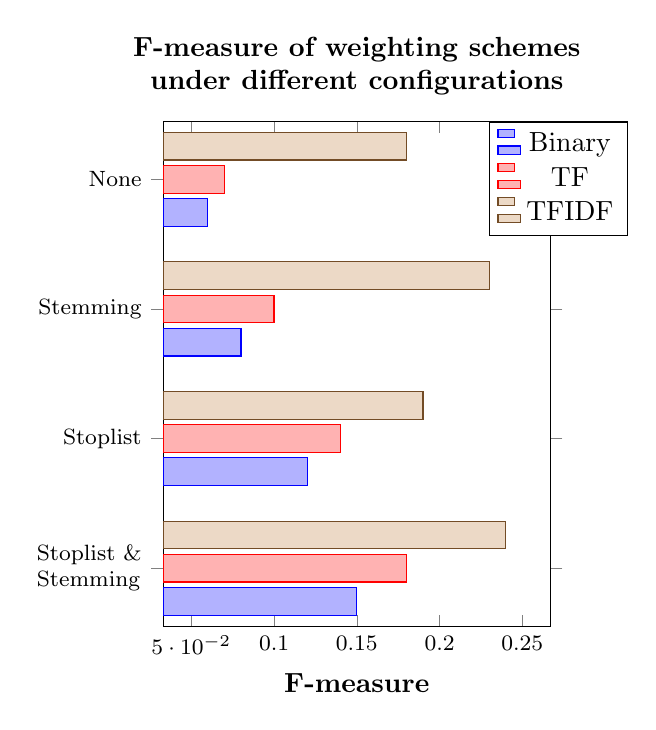
\begin{tikzpicture}[baseline]
      \begin{axis}[
          xbar,
          enlargelimits=0.15,
          legend style={at={(1.2,0.886)},anchor=east,legend columns=1},
          xlabel={\textbf{F-measure}},
          title style={align=center},
          title={\textbf{F-measure of weighting schemes} \\ \textbf{under different configurations}},
          symbolic y coords={Stoplist \&\\Stemming,Stoplist,Stemming,None},
          ytick=data,
          y tick label style={align=left}
        ]
        \addplot coordinates {(0.15,Stoplist \&\\Stemming) (0.12,Stoplist) (0.08,Stemming) (0.06,None)};
        \addplot coordinates {(0.18,Stoplist \&\\Stemming) (0.14,Stoplist) (0.10,Stemming) (0.07,None)};
        \addplot coordinates {(0.24,Stoplist \&\\Stemming) (0.19,Stoplist) (0.23,Stemming) (0.18,None)};
        \legend{Binary, TF, TFIDF}
      \end{axis}
    \end{tikzpicture}
    \captionof{figure}{F-measures of three term weighting schemes} \label{figure:f-measure}
  \end{minipage}%
  %
  \begin{minipage}{.5\textwidth}
    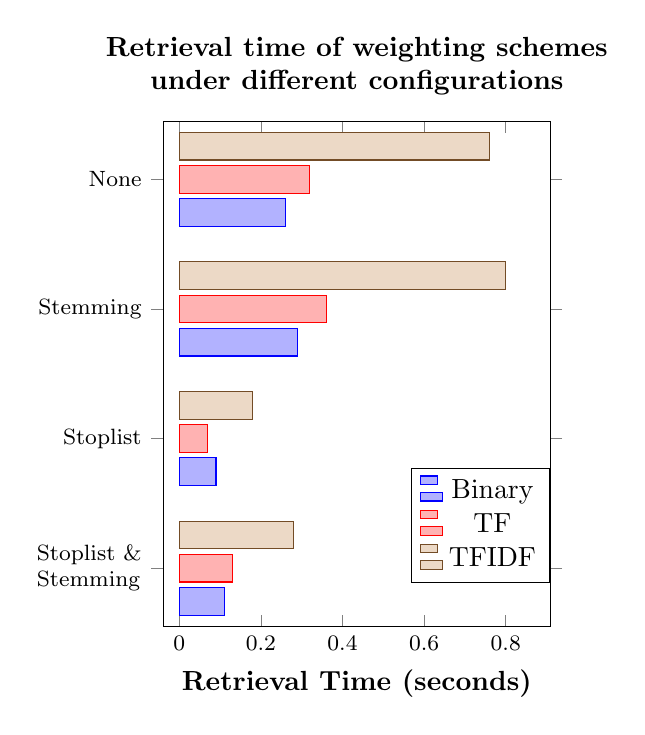
\begin{tikzpicture}[baseline]
      \begin{axis}[
          xbar,
          enlargelimits=0.15,
          legend style={at={(1,0.2)},anchor=east,legend columns=1},
          xlabel={\textbf{Retrieval Time (seconds)}},
          title style={align=center},
          title={\textbf{Retrieval time of weighting schemes} \\ \textbf{under different configurations}},
          symbolic y coords={Stoplist \&\\Stemming,Stoplist,Stemming,None},
          ytick=data,
          y tick label style={align=left}
        ]
        \addplot coordinates {(0.11,Stoplist \&\\Stemming) (0.09,Stoplist) (0.29,Stemming) (0.26,None)};
        \addplot coordinates {(0.13,Stoplist \&\\Stemming) (0.07,Stoplist) (0.36,Stemming) (0.32,None)};
        \addplot coordinates {(0.28,Stoplist \&\\Stemming) (0.18,Stoplist) (0.80,Stemming) (0.76,None)};
        \legend{Binary, TF, TFIDF}
      \end{axis}
    \end{tikzpicture}
    \captionof{figure}{Retrieval time of three term weighting schemes} \label{figure:retrieval}
  \end{minipage}
\end{figure}

\section{Discussion and Conclusion}
% Is the report a clear and accurate description of the implementation? How complete and accurate is
% the discussion of the performance of the system under a range of configurations? What inferences
% can be drawn about the performance of the IR system from these results?
According to \hyperref[figure:f-measure]{\textbf{Figure 1}}, it has been shown that TFIDF weighting
scheme has the best performance, and binary weighting scheme has the poorest performance. In
\hyperref[figure:retrieval]{\textbf{Figure 2}}, the retrival time is completely opposite, where
TFIDF weighting scheme required the longest retrieval time, and binary weighting scheme is the
overall fastest.

Based on the results in \hyperref[figure:f-measure]{\textbf{Table 1}} and
\hyperref[figure:f-measure]{\textbf{Figure 1}}, it is proved that the results will improve when
words are preprocessed by stemming and trivial words are removed using the stoplist. It is noticed
that the TFIDF weighting scheme has very small improvements when stoplist is used, but huge
performance gain when stemming is used. In contrast, binary and TF weighting scheme have larger
improvements with stoplist but smaller improvements with stemming. Reason is that the words that are
infrequent in the document collection are regarded as important in TFIDF weighting scheme, and it is
likely that an important keyword in both query and document will reduce to become a same `word'
after stemming.

According to \hyperref[figure:retrieval]{\textbf{Figure 2}}, it is proved that the retrival time
will be greatly reduced when using stoplist, but slightly increase with stemming. This is because
stemming will increase the number of common words between the query and the document, thus the
number of loops and calculations are increased which will result in a longer retrieval time. In
addition, the retrieval time is affected by code refactoring as well. Some values can be calculated
in the initialisation stage to prevent repeated calculations in the loop.

As a conclusion, the performance of the IR system could be improved by the usage of term
manipulation techniques such as stoplist and stemming. The efficiency of the IR system is mainly
affected by the implementaion approach, where sensible code refactoring could prevent repeated code
executions. Lastly, given the results shown above, it would be reasonable to choose TF over binary
weighting scheme for situations where both time and quality of results are the main priority.


\end{document}
